
一次元画像データとは,二次元(Red,Green,Blue)の画像データの列をそれぞれ足し算して,
得た3つのベクトルをくっつけることである(\ref{eq:onedimension}式参照).
$\boldsymbol R_{\rm i}$,$\boldsymbol G_{\rm i}$,$\boldsymbol B_{\rm i}$は画像データのRed,Green,Blueそれぞれの約130行目から200行目
,70行の行列,$i$は列の番号,$N$は列の数(本研究は$N$=320),$\vec u$は$1$行$960$列のベクトル.

Fig.\ref{roboteye}はロボットの視点,コース以外とロボット自分を映ってる部分がトリミングする.

\vspace{-2mm}
\begin{eqnarray}
\left\{
\begin{aligned}
\vec u_{\rm r}= \sum_{i=1}^N \boldsymbol R_{\rm i}\\
\vec u_{\rm g}= \sum_{i=1}^N \boldsymbol G_{\rm i}\\
\vec u_{\rm b}= \sum_{i=1}^N \boldsymbol B_{\rm i}\\
%begin{array}
%\vec u = \vec u_{\rm r} & \vec u_{\rm g} & \vec u_{\rm b} \\
%end{array}
\vec u = (\vec u_{\rm r},\vec u_{\rm g},\vec u_{\rm b}) \\
\end{aligned}
\right.
\label{eq:onedimension}
\end{eqnarray}


\subsubsection{大きいハンドルで教師データ収集}
教師データは,コースに障害物(他のロボット,Fig.\ref{data_colle}の黒い円囲まれてないロボット)をコースの中にランダムに置いて,
データ収集ロボットをラジコンして,障害物と壁を避けながら時計回りと反時計回り両方走行して,教師データ収集する.
障害物の位置もランダムに変更して,合計3000個教師データ収集した.

ラジコンの方法はtable\ref{radio_rule}の大きいハンドルの部分を参照して,
"D"以外のボタンを押す瞬間の画像データを一次元画像データに変更して,
ソケット通信で学習用パソコンに送信して,教師データの収集を行う.
大きいハンドルというのは,ボタン"J"と"L"押すと,
モーターの出力が35単位変えるということである.
\subsubsection{小さいハンドルで教師データ収集}
小さいハンドルで教師データ収集は大きいハンドルで教師データ収集と同じコースで収集する
,障害物については,止まってるロボット約6台,感覚運動写像より走行するロボット1台,
別の人がラジコンするロボット2台の環境で,データ収集ロボットをラジコンして,
障害物と壁を避けながら時計回りと反時計回り両方走行して,教師データ収集する.
合計6000個教師データ収集した.

ラジコンの方法はtable\ref{radio_rule}の小さいハンドルの部分を参照して,
ボタンを押す瞬間の画像データを一次元画像データに変更して,
ソケット通信で学習用パソコンに送信して,教師データの収集を行う.
小さいハンドルというのは,ボタン"J"と"L"押すと,モーターの出力が15単位変えるということである.

\begin{table}[!ht]
\setlength\tabcolsep{1pt}
\begin{center}
\begin{tabular}{|c|c|c|c|c|}
\hline
 & \multicolumn{2}{|c|}{小さいハンドル} & \multicolumn{2}{c|}{大きいハンドル}\\
\hline
 & Left motor & Right motor & Left motor & Right motor \\
\hline
W & +20 & +20 & +35 & +35\\
\hline
S & -15 & -15 & -35 & -35\\
\hline
A & * & * & -56 & -56\\
\hline
D & * & * & =0 & =0 \\
\hline
J & -15 & +15 & -0 & +35 \\
\hline
L & +15 & -15 & +35 & -0 \\
\hline
K & \multicolumn{4}{|c|}{操作JとKで変化した出力が0になる} \\
\hline
\end{tabular}
\end{center}
\caption{
大きいハンドルと小さいハンドルの違い
}
\label{radio_rule}
\end{table}



\vspace{-2mm}
\begin{figure}[h]
        \centering
        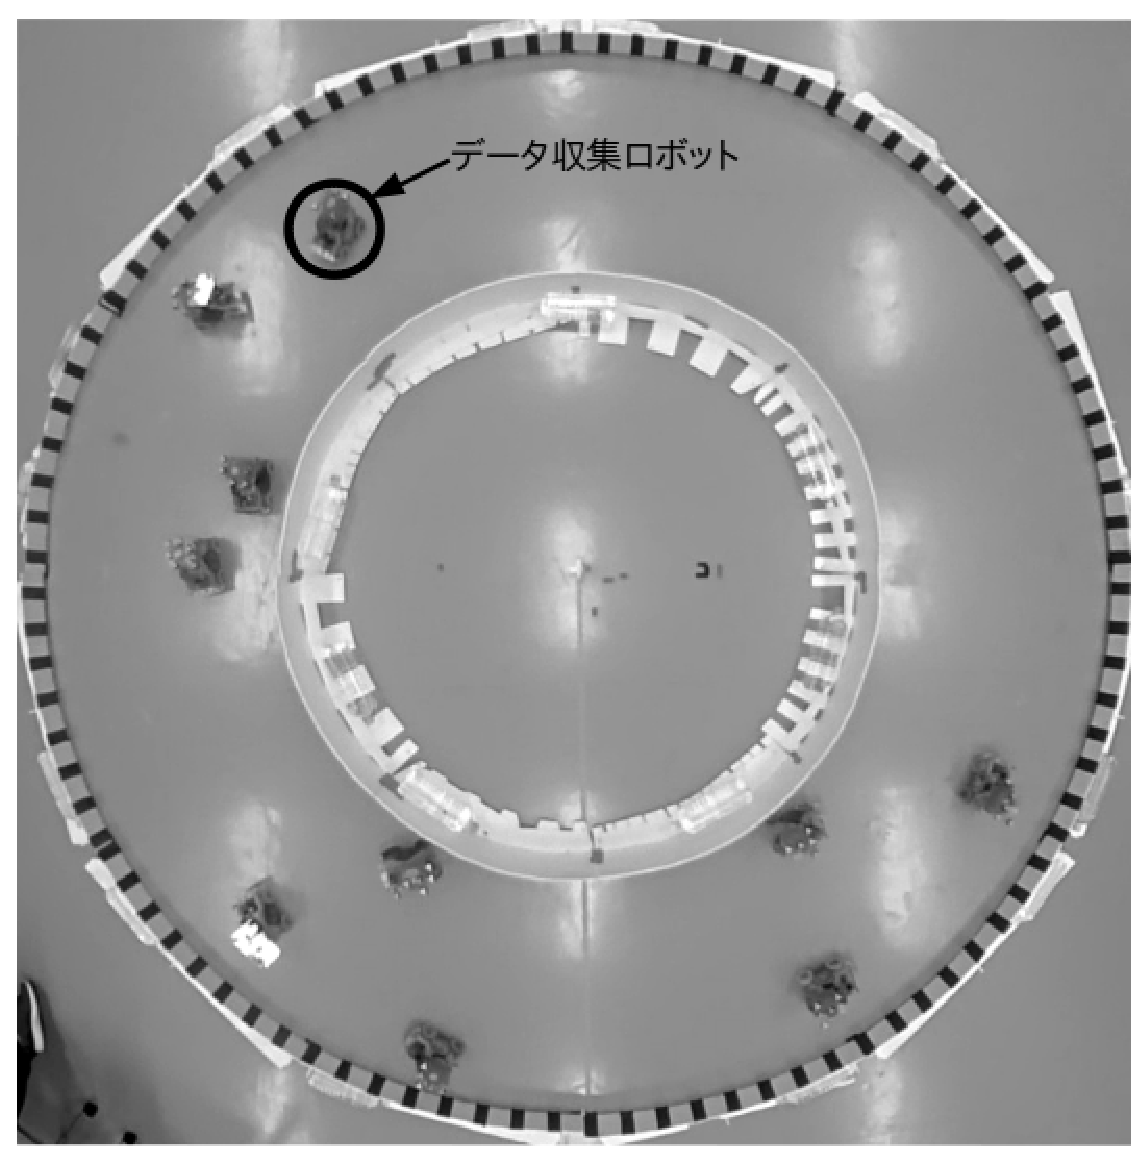
\includegraphics[width=0.8\linewidth]{teacher_collection.eps}
        \caption{データ収集}
        \label{data_colle}
\end{figure}

\vspace{-5mm}
\begin{figure}[h]
\centering
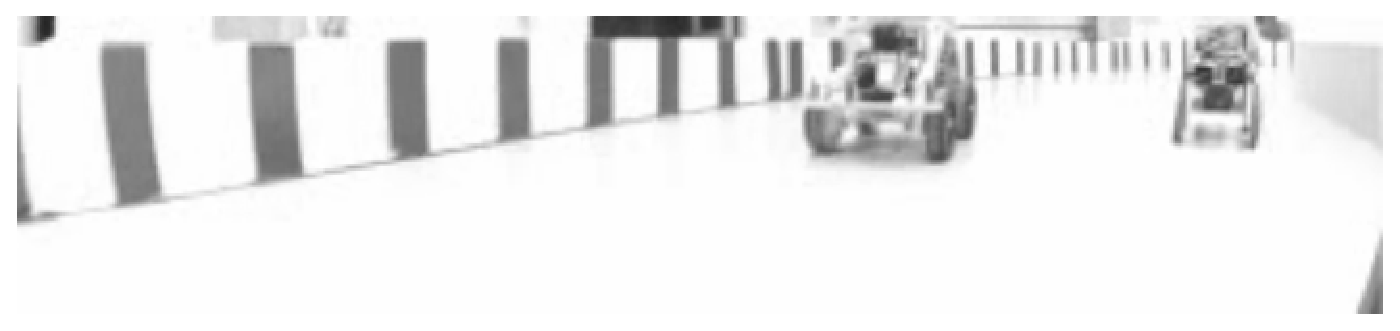
\includegraphics[width=0.7\linewidth]{robot_eye.eps}
\caption{ロボットの視点}
\label{roboteye}
\end{figure}



